\documentclass[12pt]{article}

\usepackage{fontspec}
\usepackage{hyperref}
\usepackage[separate-uncertainty=true,load=addn]{siunitx}
\usepackage{float}
\usepackage[tableposition=top]{caption}
\usepackage[margin=1in]{geometry}
\usepackage[citestyle=ieee,sorting=none,backend=biber]{biblatex}
\usepackage[affil-it]{authblk}

\graphicspath{ {images/} }
\addbibresource{test.bib}

\newcommand{\specialcell}[2][c]{%
  \begin{tabular}[#1]{@{}c@{}}#2\end{tabular}}

\floatstyle{plaintop}

\setmainfont{Times New Roman}

\title{Semiconductor Detectors}
\author{J.R. Powers-Luhn}
\date{April 27, 2017}

\affil{NE550, Thursday 17:30}

\renewcommand{\baselinestretch}{1.5}
%\setlength{\baselineskip}{0.5em}

\begin{document}
%\linespread{1.5}

\maketitle

\section{Abstract}
The performance of two different types of semiconductor detectors, High Purity Germanium (HPGE) and Cadmium Zinc Telluride (CZT), were examined and compared for a variety of pure, sealed sources. Calculations were made for the resolution of known peaks (using a gaussian curve fitting technique), linearity of response to radiation (via a linear least-squares fit to well characterized sources), and photopeak response for each detector material. In addition, an attempt was made to examine the geometric efficiency of the HPGe detector as a function of distance from a near point source, with qualitative evaluation of the impact of deadtime. Spectra for an assortment of sources and detectors are provided with notable features identified on their plots.

\section{Introduction}
Semiconductor detectors are useful for collecting detailed spectra for radiation sources. Their higher density (HPGe has a density of \SI{5.32}{\gram\per\centi\meter^2} \cite{giaz}) allows much smaller detectors than gas detectors, with the additional advantage of shorter deadtimes. Additionally, they exhibit dead times significantly lower than gas detectors, often by several orders of magnitude \cite{textbook}. Furthermore, in contrast to scintillation detectors, they do not require the use of coupled photomultiplier tubes with the efficiency losses implied.

Semiconductor detectors have electrons that occupy outer shells below the conduction band when they are at rest. When they are biased with an appropriate voltage, the gap between the valence band and the conduction band shrinks to a value that can be bridged by the introduction of ionizing radiation. These band gaps tend to be low--1.572 eV for CZT at 300K \cite{bandgap}. This can introduce additional problems in very sensitive materials such as HPGe, where thermal excitations can cause increased noise due to spontaneous conduction (without an inciting ionizing event). As a result, HPGe detectors must be cooled by liquid nitrogen or by complicated mechanical cooling means.

While the semiconductor detectors are generally very performant, they are not identical. The size of the band gap, and therefore the resolution that they can provide, varies from material to material. Additionally, different materials exhibit different cross sections for various ranges of radiation, meaning that they have different responses to ionizing events. These changes introduce various tradeoffs that must be made between detector materials, including convenience and price in addition to efficiency and resolution.

In order to characterize the latter two tradeoffs, measurements were made for an assortment of sealed sources with known spectra using two types of detectors: high purity Germanium and Cadmium Zinc Telluride. These spectra were taken with a standardized chain of nuclear instrumentation and Maestro MCA software. A moderately-well characterized background was taken in order to directly compare the response of the detectors.

\section{Experimental}
\subsection{MCA Linearity}
In order to determine the linearity response of the ORTEC 927 ASPEC MCA, a model BNC BL-2 voltage pulse generator was connected through an ORTEC 572A amplifier to the MCA while the output of the pulse generator was also monitored via an GW INSTEK model GDS-3254 oscilloscope, as indicated in figure \ref{fig:MCAblock}. The output of the MCA was recorded in the Maestro software for several voltage settings, and the channels corresponding to each peak recorded.

\begin{center}
\begin{figure}
	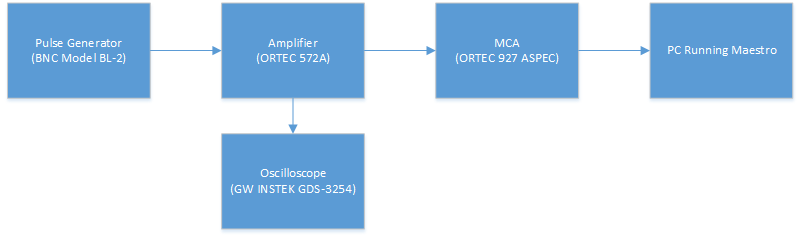
\includegraphics[width=\linewidth]{block1}
	\caption{MCA experiment block diagram}
	\label{fig:MCAblock}
\end{figure}
\end{center}

\subsection{MCA Dead Time}
In order to determine the dead time of the MCA, the pulse generator was then set to produce a double pulse with a \SI{3}{\micro\second} rise time and a \SI{10}{\micro\second} fall time. Amplifier shaping time was set to \SI{0.5}{\micro\second} with an amplitude of \SI{5.44}{\volt}. The MCA was set to conduct a continuous collection with a 12 bit conversion gain. The spacing between the pulse was adjusted and the threshold at which the MCA was able to distinguish between the pulses (the point at which two peaks appeared on the spectrum) recorded. 

\subsection{HPGe Evaluation}
The MCA was then connected to an HPGe/Preamplifier/Amplifier chain as indicated in figure \ref{fig:hpgeblock}. The amplifier shaping time was set to \SI{10}{\micro\second} with a gain setting of 10 and unipolar output. After a \SI{10}{\minute} background was collected, an assortment of sealed sources were placed at a distance of approximately \SI{10}{\centi\meter} from the detector face. Information regarding the sources is presented in table \ref{tab:hpgesources}. Spectra for these sources were collected in the highest-available number of channels (14 bits) in order to take advantage of the high resolution of the HPGe detector. Sources were counted for \SI{150}{\second} in order to obtain sufficient counts to obtain reasonable statistics.

\begin{center}
\begin{figure}
	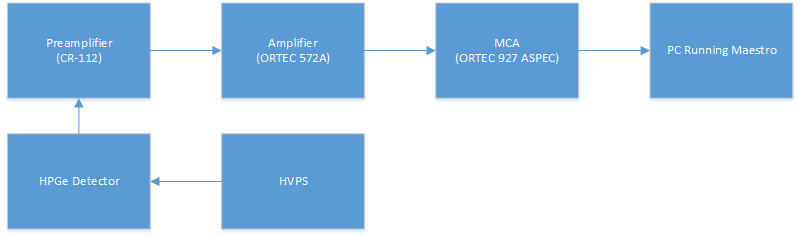
\includegraphics[width=\linewidth]{block2}
	\caption{HPGe experiment block diagram}
	\label{fig:hpgeblock}
\end{figure}
\end{center}

\begin{center}
\begin{table}
	\centering
	\caption{Sources for HPGe Evaluation\label{tab:hpgesources}}
	\begin{tabular}{c c c}
		\hline\hline
		Source & Date & Activity \\
		\hline
		Na-22 & April 2015 & \SI{1}{\micro\curie} \\
		Cs-137 & April 2015 & \SI{10}{\micro\curie} \\
		Co-60 & May 2012 & \SI{1}{\micro\curie} \\
		Mn-54 & February 2012 & \SI{10}{\micro\curie} \\
		Cd-109 & May 2015 & \SI{1}{\micro\curie} \\
		Ba-133 & February 2012 & \SI{1}{\micro\curie} \\
		Co-57 & May 2015 & \SI{1}{\micro\curie} \\
		\hline
	\end{tabular}
\end{table}
\end{center}

\subsection{HPGe Geometric variation}
A \SI{1}{\micro\curie} Cs-137 source dated February 2012 was used to determine the response of the HPGe detector to sources at various ranges. The source was placed in a holder above the detector face. A \SI{150}{\second} spectrum was recorded on contact and at heights of \SI{2.6\pm.3}{\centi\meter}, \SI{6.2\pm.3}{\centi\meter}, \SI{9.4\pm.3}{\centi\meter}, \SI{11.5\pm.3}{\centi\meter}, and \SI{14.7\pm.3}{\centi\meter}.

\subsection{CZT Evaluation}
An effort was made to objectively compare the HPGe detector to another type of detector, namely a Cadmium Zinc Telluride (CZT) detector. This data collection was performed by the course instructors, so precise settings for the electronics chain were not available at the time of this report. The information that was available for this experiment is recorded in table \ref{tab:cztsources}.

\begin{center}
\begin{table}
	\centering
	\caption{Sources and count time for CZT evaluation\label{tab:cztsources}}
	\begin{tabular}{c c}
		\hline\hline
		Source & Count time (\si{\second}) \\
		\hline
		Na-22 & 300 \\
		Co-57 & 300 \\
		Co-60 & 600 \\ 
		Cd-109 & 300 \\
		Ba-133 & 300 \\
		Cs-137 & 120 \\
		\hline
	\end{tabular}
\end{table}
\end{center}

\section{Results}
\subsection{MCA performance}

\subsection{HPGe Resolution and efficiency}
The spectra from the assorted sources were analyzed using Python and the PeakUtils library \cite{peakutils} in order to determine a relationship between channel number and energy. The detected peaks were correlated to known gamma emission spectra for these sources and a linear fit was performed on this data. A plot of the data and the linear fit can be seen in figure \ref{fig:hpgeenergytochannel}. Based on the $R^2>0.9999$ value, it was determined that further analysis could be conducted in terms of energy vice channel number, and the spectra were converted accordingly.

The spectrum for the Na-22 source showed significant photopeaks, as expected (see figure \ref{fig:na22hpge}). The principle gamma emission from the Na-22 source is visible at E=\SI{1274 \pm 0.1}{\kilo\electronvolt}, (see equation \ref{eqn:annhilationenergy}). The largest peak in this spectrum corresponded to the annhilation of the positrons from the source, corresponding to an energy of \SI{511}{\kilo\electronvolt}. These gamma rays produced secondary scattering events via the process of Compton Scattering. This process produced a continuous spectrum (due to the three-body nature of the products of Compton Scattering event), the maximum energy (see equation \ref{eqn:compton}) produces an observable drop in the energy which corresponds to the maximum energy of the scattered electrom from these events. This is visible as a "Compton Edge" \cite{textbook}. This feature appears to one degree or another in most of the spectra recorded for this report.

\begin{center}
\begin{figure}
	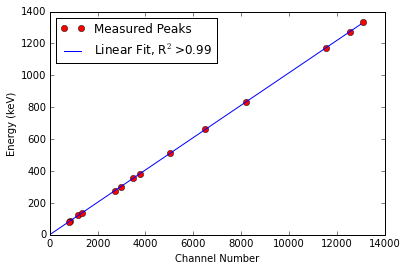
\includegraphics{hpge_energy_linearity}
	\caption{HPGe Energy/Channel Relationship}
	\label{fig:hpgeenergytochannel}
\end{figure}
\end{center}

\begin{center}
\begin{figure}
	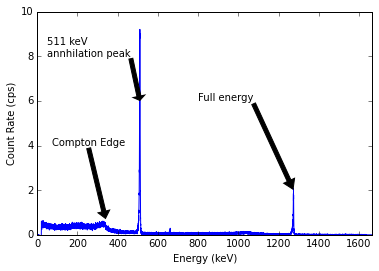
\includegraphics{hpge_na22}
	\caption{Na-22 emission spectrum for HPGe detector}
	\label{fig:na22hpge}
\end{figure}
\end{center}

\begin{equation}
	\label{eqn:annhilationenergy}
	E_\gamma = m_e \times c^2 = \SI{511}{\kilo\electronvolt}
\end{equation}

\begin{equation}
	\label{eqn:compton}
	E_s^{Max} = E_\gamma \left(1 - \frac{1}{1 + \frac{2E_\gamma}{m_e c^2}} \right)
\end{equation}

The spectrum for the Mn-54 source (see figure \ref{fig:mn54hpge}) showed a single peak at \SI{835}{\kilo\electronvolt} and no other visible features. This corresponds to its electron capture decay, which occurs with a branching frequency of greater than 0.9999 \cite{nucdata}.

\begin{center}
\begin{figure}
	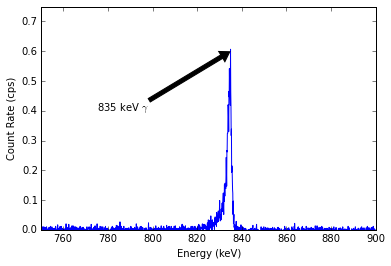
\includegraphics{hpge_mn54}
	\caption{Mn-54 emission spectrum for HPGe detector}
	\label{fig:mn54hpge}
\end{figure}
\end{center}

Two isotopes of Cobalt were examined, Co-57 and Co-60. Co-57 decays via several modes, only three of which have significant branching fractions (>1\%). The lowest energy of these, an electron capture at \SI{14.4}{\kilo\electronvolt} was low enough energy that it was not visible in the background-corrected spectrum (due to the prevalence of X-rays in the low-energy region below approximately \SI{20}{\kilo\electronvolt}). The remaining two peaks are closely spaced at \SI{122}{\kilo\electronvolt} and \SI{136}{\kilo\electronvolt}, making them a good mechanism to evaluate the resolution of a detector. As expected, the two peaks were distinct on the plotted spectrum, as can be seen in figure \ref{fig:co57hpge}. The distinct peaks also provide the opportunity to qualitatively verify the branching ratios. The magnitudes of a gaussian fit to the \SI{122}{\kilo\electronvolt} and \SI{136}{\kilo\electronvolt} were 15.7 cps and 1.9 cps respectively. The ratio of these values, \num{8.3 \pm 0.5}, is within error of their given branching ratios, 85.6 / 10.7 = 8.01 \cite{nucdata}.

\begin{center}
\begin{figure}
	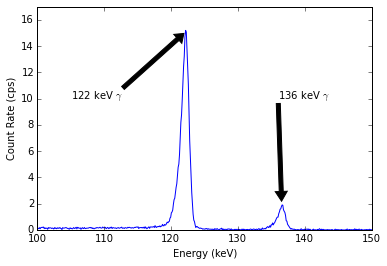
\includegraphics{hpge_co57}
	\caption{Co-57 emission spectrum for HPGe detector}
	\label{fig:co57hpge}
\end{figure}
\end{center}

The spectrum for Co-60 (figure \ref{fig:co60hpge}) shows the expected peaks at \SI{1174}{\kilo\electronvolt} and \SI{1332}{\kilo\electronvolt}. These peaks should show up with equal branching ratios but instead display a ratio of \num{1.20 \pm 0.14}. Further analysis is appropriate to determine if this reflects a difference in the efficiency of these peaks as this experiment showed the detector photoefficiencies at these energies to be 0.0043 and 0.0036 respectively (see table \ref{tab:hpgeperf}).

\begin{center}
\begin{figure}
	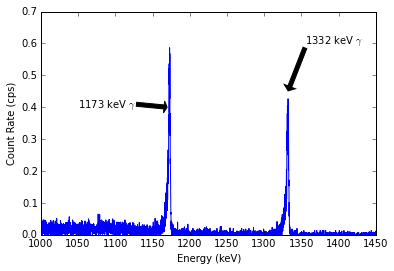
\includegraphics{hpge_co60}
	\caption{Co-60 emission spectrum for HPGe detector}
	\label{fig:co60hpge}
\end{figure}
\end{center}

Cadmium 109 (figure \ref{fig:cd109hpge}) produced the expected peak at \SI{88.04}{\kilo\electronvolt} and little else of note.

\begin{center}
\begin{figure}
	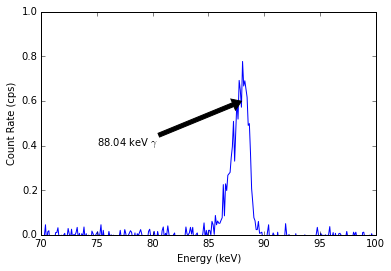
\includegraphics{hpge_cd109}
	\caption{Cd-109 spectral for HPGe detector}
	\label{fig:cd109hpge}
\end{figure}
\end{center}

Barium 133 (figure \ref{fig:ba133hpge}) had five discernable peaks at \SIlist{81;276;303;356;384}{\kilo\electronvolt}.

\begin{center}
\begin{figure}
	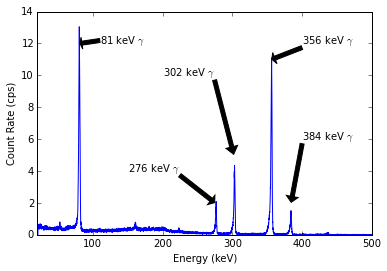
\includegraphics{hpge_ba133}
	\caption{Ba-133 spectral for HPGe detector}
	\label{fig:ba133hpge}
\end{figure}
\end{center}

Cs-137 exhibited a strong peak at \SI{662}{\kilo\electronvolt}. In addition, the plot in figure \ref{fig:cs137hpge} showed not just a compton edge at \SI{477}{\kilo\electronvolt} but also the full range of the compton continuum, higlighted in the figure.

\begin{center}
\begin{figure}
	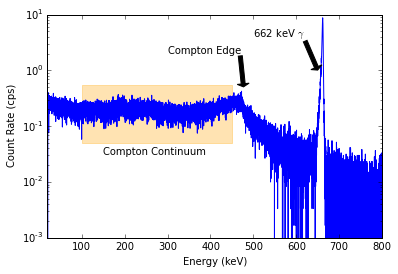
\includegraphics{hpge_cs137}
	\caption{Cs-137 spectral for HPGe detector}
	\label{fig:cs137hpge}
\end{figure}
\end{center}

In order to determine the detector efficiency for each of the photopeaks from the sources, the spectral data representing each of the peaks were segregated out and treated separately for this portion. For each prominent spectral feature, an attempt was made to determine the resolution of the detector chain for that energy. In order to conduct this analysis, a gaussian curve of arbitrary amplitude was fit to the data near the peak. The fitted amplitude represented the photopeak amplitude; the fitted $\sigma$ was used with equation \ref{eqn:resolution} \cite{textbook} to determine the FWHM of the peak (corresponding to the resolution of the detector). The results of this analysis are recorded in table \ref{tab:hpgeperf}.

\begin{equation}
	FHWM = 2 \sigma \sqrt{2 \ln{2}}
	\label{eqn:resolution}
\end{equation}

\begin{center}
\begin{table}
	\centering
	\caption{Efficiency of HPGe Detector\label{tab:hpgeperf}}
	\begin{tabular}{c c c c c c}
		\hline\hline
		Source & \specialcell{Energy\\($\pm$ \SI{0.1}{\kilo\electronvolt})} & \specialcell{FWHM\\(\si{\kilo\electronvolt})} & \specialcell{Photopeak\\(cps $\times$ \si{\kilo\electronvolt})} & \specialcell{Total\\(cps $\times$ \si{\kilo\electronvolt})} & Photopeak efficiency \\
		\hline
		Na-22  &  511  & 2.83 &  25.4 & 2339  & 0.011 \\
		       & 1274  & 2.75 &  4.48 & 2339  & 0.0019 \\
		Mn-54  &  835  & 1.73 & 0.861 &  82.5 & 0.010 \\
		Co-57  &  122  & 1.05 &  15.7 & 413.2 & 0.038 \\
               &  136  & 1.06 &  1.90 & 413.2 & 0.0046 \\
        Co-60  & 1173  & 2.25 &  1.07 & 250.4 & 0.0043 \\
               & 1332  & 2.32 & 0.893 & 250.4 & 0.0036 \\
        Cd-109 & 88.04 & 1.22 & 0.882 & 42.65 & 0.021  \\
        Ba-133 & 81    & 1.51 & 19.47 & 1509  & 0.013 \\
               & 276   & 1.36 & 2.520 & 1509  & 0.0017 \\
               & 303   & 1.36 & 5.613 & 1509  & 0.0037 \\
               & 356   & 1.41 & 15.03 & 1509  & 0.010 \\
               & 384   & 1.53 & 2.109 & 1509  & 0.0014 \\
        Cs-137 & 662   & 1.82 & 15.33 & 1334 & 0.011 \\
		\hline
	\end{tabular}
\end{table}
\end{center}

In order to examine the geometric response of the HPGe detector, spectra were taken for a Cs-137 source at a variety of distances. These spectra are shown in figure \ref{fig:cs137heights}. These spectra show that the height of the peak as compared to the height of other features (notably the compton edge and continuum) shrinks at short distances, indicating high deadtime. In fact, the on-contact deadtime was 87\%, as compared to a deadtime of 1.7\% for a height of \SI{14.7}{\centi\meter}.

\subsection{CZT Performance}
A similar analysis to that described for the HPGe detector above was applied to the spectra recorded by class staff for a Cadmium Zinc Telluride detector. These can be seen in figures \ref{fig:na22czt}, \ref{fig:co57czt}, \ref{fig:co60czt}, \ref{fig:cd109czt}, \ref{fig:ba133czt}, and \ref{fig:cs137czt}. Prominent features are identified in the figures and the results of resolution and efficiency calculations are provided in table \ref{tab:cztfwhm}. It was immediately apparent that the CZT detector had significantly lower resolution than the HPGe detector, with many spectral features either weakly present or invisible. As a result, the calculations had to be made with far fewer peaks. The peaks that were available, however, made for a still-excellent energy to channel number relationship, as seen in figure \ref{fig:cztenergy}.

\begin{center}
\begin{figure}
	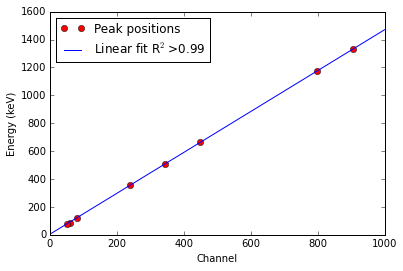
\includegraphics{czt_energy_linearity}
	\caption{CZT Energy/Channel relationship}
	\label{fig:cztenergy}
\end{figure}
\end{center}

\begin{center}
\begin{figure}
	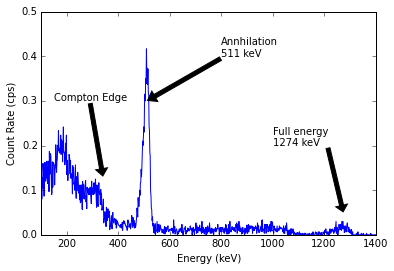
\includegraphics{czt_na22}
	\caption{Na-22 spectrum for CZT detector}
	\label{fig:na22czt}
\end{figure}
\end{center}

\begin{center}
\begin{figure}
	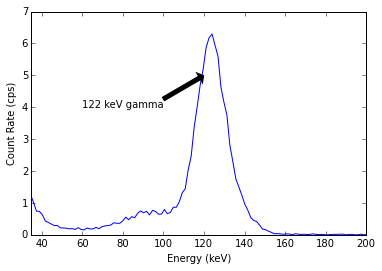
\includegraphics{czt_co57}
	\caption{Co-57 spectrum for CZT detector}
	\label{fig:co57czt}
\end{figure}
\end{center}

\begin{center}
\begin{figure}
	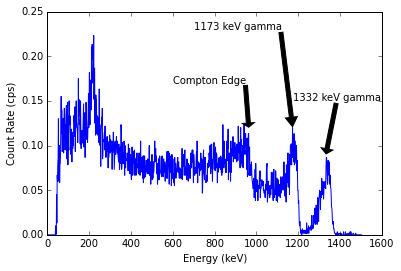
\includegraphics{czt_co60}
	\caption{Co-60 spectrum for CZT detector}
	\label{fig:co60czt}
\end{figure}
\end{center}

\begin{center}
\begin{figure}
	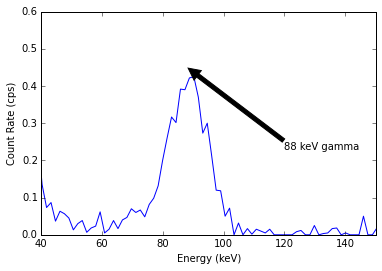
\includegraphics{czt_cd109}
	\caption{Cd-109 spectrum for CZT detector}
	\label{fig:cd109czt}
\end{figure}
\end{center}

\begin{center}
\begin{figure}
	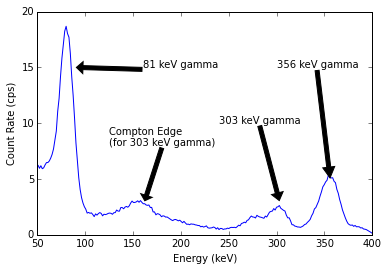
\includegraphics{czt_ba133}
	\caption{Ba-133 spectrum for CZT detector}
	\label{fig:ba133czt}
\end{figure}
\end{center}

\begin{center}
\begin{figure}
	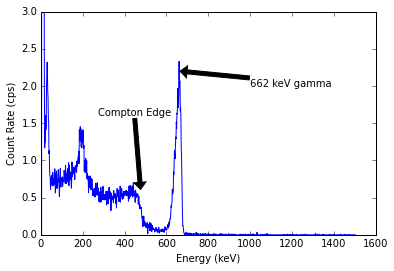
\includegraphics{czt_cs137}
	\caption{Cs-137 spectrum for CZT detector}
	\label{fig:cs137czt}
\end{figure}
\end{center}

\begin{center}
\begin{table}
	\centering
	\caption{Efficiency of CZT Detector\label{tab:cztfwhm}}
	\begin{tabular}{c c c c c c}
		\hline\hline
		Source & \specialcell{Energy\\($\pm$ \SI{0.1}{\kilo\electronvolt})} & \specialcell{FWHM\\(\si{\kilo\electronvolt})} & \specialcell{Photopeak\\(cps $\times$ \si{\kilo\electronvolt})} & \specialcell{Total\\(cps $\times$ \si{\kilo\electronvolt})} & Photopeak efficiency \\
		\hline
		Na-22 & 511 & 21.7 & 8.17 & 50.8 & 0.16 \\
		 & 1274 & 50.0 & 0.89 & 50.8 & 0.018 \\
		Co-57 & 122 & 13.5 & 85 & 111 & 0.77 \\
		Co-60 & 1173 & 60.1 & 5.7 & 71.51 & 0.080 \\
		& 1332 & 43.2 & 3.13 & 0.044 \\
		Cd-109 & 88.04 & 11.4 & 4.94 & 13.10 & 0.38 \\
		Ba-133 & 80.99 & 20.7 & 349 & 880 & 0.40 \\
		& 356 & 19.7 & 106 & 880 & 0.12 \\
		Cs-137 & 662 & 23.6 & 49.3 & 4314 & 0.011 \\
		\hline
	\end{tabular}
\end{table}
\end{center}

\section{Conclusion}
The ORTEC 927 ASPEC MCA was determined to perform within the ranges required for spectral analysis, with sufficient resolution and linear response at a variety of input voltages. The performance of an HPGe detector was analyzed for a variety of well-characterized sources. Its resolution was found to be excellent, with full-width, half-max (FWHM) typically in the range of 1-3 (see table \ref{tab:hpgeperf}). A CZT detector was also analyzed which displayed FWHM values 10-20x larger than the HPGe detector, but with photoefficiencies that were higher than the HPGe by approximately the same magnitude. This fit with the findings of Perez-Andujar, et al \cite{perez-andujar}. Some statistical analysis was applied for error propogation purposes, but it would be instructive to collect more data in the future in more controlled scenarios in order to more directly compare these two detectors. Specifically, the collection times for the CZT detector were significantly longer, and the reasons for this were not clear as this data was provided to the author rather than collected directly.

\printbibliography


\end{document}